% Fig. 1 (pipeline). Build: pdflatex fig_pipeline.tex  ->  fig_pipeline.pdf
\documentclass[border=2pt]{standalone}
\usepackage{mathptmx}
\usepackage{tikz}
\usetikzlibrary{arrows.meta}
\begin{document}
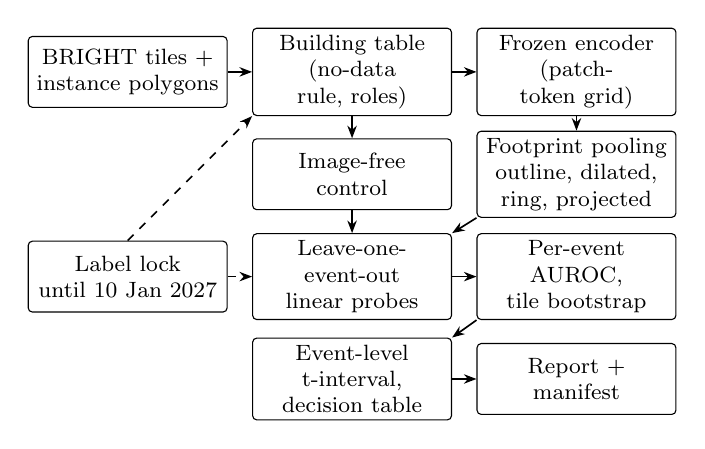
\begin{tikzpicture}[
  box/.style={draw, rounded corners=1.5pt, align=center, font=\footnotesize, inner sep=2.5pt,
              minimum height=9mm, text width=2.35cm},
  arr/.style={-{Stealth[length=1.6mm]}, semithick}]
\def\cx{2.85}\def\cy{1.3}
\node[box] (data)  at (0,0)         {BRIGHT tiles +\\ instance polygons};
\node[box] (table) at (\cx,0)       {Building table\\ (no-data rule, roles)};
\node[box] (enc)   at (2*\cx,0)     {Frozen encoder\\ (patch-token grid)};
\node[box] (free)  at (\cx,-\cy)    {Image-free\\ control};
\node[box] (pool)  at (2*\cx,-\cy)  {Footprint pooling\\ outline, dilated,\\ ring, projected};
\node[box] (lock)  at (0,-2*\cy)    {Label lock\\ until 10 Jan 2027};
\node[box] (probe) at (\cx,-2*\cy)  {Leave-one-event-out\\ linear probes};
\node[box] (auc)   at (2*\cx,-2*\cy){Per-event AUROC,\\ tile bootstrap};
\node[box] (stats) at (\cx,-3*\cy)  {Event-level t-interval,\\ decision table};
\node[box] (rep)   at (2*\cx,-3*\cy){Report +\\ manifest};
\draw[arr] (data) -- (table);
\draw[arr] (table) -- (enc);
\draw[arr] (enc) -- (pool);
\draw[arr] (table) -- (free);
\draw[arr] (free) -- (probe);
\draw[arr] (pool.south west) -- (probe.north east);
\draw[arr] (probe) -- (auc);
\draw[arr] (auc.south west) -- (stats.north east);
\draw[arr] (stats) -- (rep);
\draw[arr, dashed] (lock) -- (probe);
\draw[arr, dashed] (lock.north) -- (table.south west);
\end{tikzpicture}
\end{document}
